\begin{figure}[tp]
    \centering
    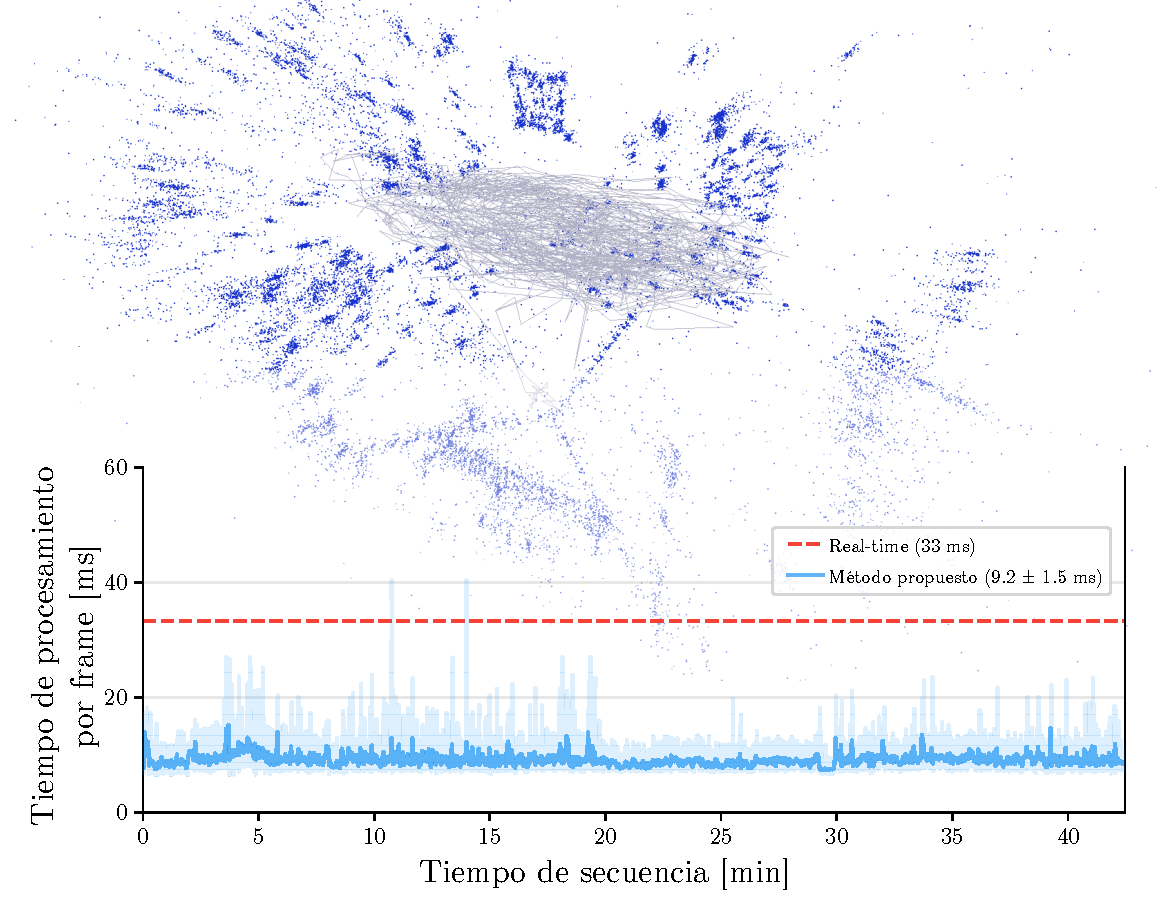
\includegraphics[width=1\linewidth]{images/abstract.mgo12.pdf}
    \caption{En la parte superior, un mapa de puntos generados por el sistema propuesto en la secuencia MGO12, de más de 40 minutos y cuatro cámaras, del Monado SLAM Dataset. En la parte inferior, una gráfica del tiempo de procesamiento por frame para esa secuencia. Se observa que el método opera por debajo del límite de tiempo real.}
    \label{fig:abstract-image}
\end{figure}

% PROBLEMA GENERAL
Los sistemas de robótica móvil y realidad virtual/aumentada (VR/AR) modernos operan frecuentemente
en plataformas con recursos computacionales y energéticos estrictamente acotados, como
nano drones (NAVs), robots móviles y headsets de VR/AR. Un sistema ineficiente no solo degrada la experiencia de usuario o el rendimiento del robot, sino que implica baterías más grandes, comprometiendo la viabilidad del sistema. Esto exige soluciones que operen en tiempo real sin depender de
hardware especializado como GPUs. Los métodos de SLAM geométricos son una alternativa
validada para entornos embebidos \cite{galagain2025semanticslamreadyembedded}. Sin embargo, cumplir
con los requisitos de tiempo real sigue siendo un desafío abierto: incluso sistemas VIO del
estado del arte presentan dificultades para garantizar robustez y procesamiento en tiempo real en
condiciones realistas \cite{demayo2025monadoslamdataset}. El desafío central es lograr precisión, eficiencia computacional y robustez, condiciones necesarias para ser desplegable en la práctica.

% VI-SLAM
La odometría visual-inercial (VIO) y el VI-SLAM fusionan cámaras
e IMU: la IMU provee estimaciones de alta frecuencia del movimiento mientras que las
cámaras aportan información rica del entorno, permitiendo estimaciones de pose precisas y
robustas ante condiciones desafiantes. El VI-SLAM además de estimar la localización, incorpora un mapa
persistente que habilita la detección de ciclos (loop closure) para corregir el drift acumulado y la reutilización del mapa, capacidades esenciales para una operación prolongada.

% OBJETIVO PRINCIPAL Y MÉTODO
El objetivo principal de este trabajo es desarrollar un sistema de VI-SLAM que aborde las limitaciones mencionadas. El método propuesto está basado en Basalt \cite{usenko2020basalt}, un sistema VIO del estado del arte para VR/AR, y es una extensión del trabajo \cite{zanotti2024basaltxr}, al que se le incorpora un mapa persistente y múltiples mejoras detalladas en la Sección \ref{sec:method}.

% CONTRIBUCIONES
El sistema propuesto extiende Basalt con un mapa persistente gestionado de manera inteligente, detección y cierre de ciclos con técnicas eficientes, y bundle adjustment adaptado de \textit{Structure from Motion} (SfM). Las principales contribuciones son:
\begin{itemize}
    \item Una extensión de Basalt con mapa persistente, cuya arquitectura basada en comunicación asíncrona entre componentes evita que las operaciones costosas del mapa degraden el rendimiento del sistema. Incorpora dos nuevos componentes que interactúan con el back-end de Basalt e implementan: detección de ciclos mediante HashBoW \cite{hashbow2024stricker} para recuperar eficientemente keyframes de contenido similar; optimización liviana del mapa mediante \textit{Pose Graph Optimization} para corregir el error acumulado luego de las detecciones de ciclos; fusión de mapa para asociar datos a largo plazo; y culling de keyframes para mantener el tamaño del mapa acotado, con heurísticas que priorizan keyframes de alta calidad visual y utilidad para la consistencia global.
    \item Un método eficiente y numéricamente estable de bundle adjustment para optimizar mapas resultantes de sistemas VI-SLAM multicámara con modelos de cámara arbitrarios. Se basa en RootBA \cite{demmelBasaltSquareRoot2021a}, que formula el problema mediante factorización QR, siguiendo la línea de \cite{demmelBasaltSquareRoot2021}, que lo aplicó por primera vez en la optimización local de Basalt.
    \item Una evaluación exhaustiva del sistema propuesto sobre datasets con amplia variedad de escenarios y desafíos típicos de robótica y VR/AR, en la que se mide rigurosamente la precisión y el rendimiento comparándolo con dos alternativas del estado del arte.
\end{itemize}

% CLAIMS
En resumen, el sistema alcanza una precisión comparable al estado del arte, principalmente en entornos típicos de VR/AR. También, es robusto ante condiciones desafiantes, como escenarios de baja textura, y mantiene la operación en tiempo real incluso en trayectorias de larga duración. Por último, el método de bundle adjustment propuesto es numéricamente estable y admite ejecución en precisión simple, lo que se traduce en una mejora de rendimiento considerable.
